\documentclass[10pt,a4paper,twocolumn]{article}
\usepackage[T1]{fontenc}
\usepackage[utf8]{inputenc}
\usepackage{lmodern}
\usepackage[a4paper,margin=18mm,bottom=20mm]{geometry}
\usepackage{amsmath,amssymb,bm}
\usepackage{graphicx}
\usepackage{booktabs}
\usepackage{microtype}
\usepackage[numbers,sort&compress]{natbib}
\usepackage{url}
\usepackage[hidelinks]{hyperref}
\hypersetup{pdftitle={Copper powder NMR in anilite Cu7S4: quadrupolar constraints and reassignment of earlier NQR spectra}}
\setlength{\columnsep}{6mm}
\setlength{\parindent}{1em}
\setlength{\parskip}{0pt}
\setlength{\textfloatsep}{10pt}
\setlength{\dbltextfloatsep}{11pt}
\setlength{\floatsep}{8pt}
\renewcommand{\topfraction}{0.9}
\renewcommand{\dbltopfraction}{0.9}
\renewcommand{\textfraction}{0.08}
\renewcommand{\floatpagefraction}{0.8}
\renewcommand{\dblfloatpagefraction}{0.8}
\setcounter{topnumber}{3}
\setcounter{dbltopnumber}{3}
\raggedbottom
\newcommand{\Cu}{\mathrm{Cu}}
\newcommand{\nqr}{\mathrm{NQR}}
\newcommand{\nuz}{\nu_{\mathrm Z}}
\newcommand{\nuq}{\nu_Q}
\newcommand{\twe}{T_{2e}}
\newcommand{\units}[1]{\,\mathrm{#1}}
\begin{document}
\lefthyphenmin=3
\righthyphenmin=3
\hyphenation{NMR NQR EFG EFGs}

\twocolumn[%
\begin{center}
{\LARGE\bfseries Copper powder NMR in anilite Cu$_7$S$_4$: quadrupolar constraints and reassignment of earlier NQR spectra\par}
\vspace{6pt}
{\small Working manuscript --- 27 November 2026\par}
\vspace{10pt}
\begin{minipage}{0.94\textwidth}
\small
\textbf{Abstract.}
Copper spin-echo nuclear magnetic resonance (NMR) spectra of an unoriented powder identified as anilite, Cu$_7$S$_4$, are analyzed together with nuclear quadrupole resonance (NQR) data previously obtained on the same material. The relevant phase was originally described as geerite and subsequently as digenite; repeat X-ray diffraction before the NMR measurements established its anilite identity. Narrow resonances of metallic copper in the probe are treated as instrumental contributions. Exact diagonalization of the spin-$3/2$ Hamiltonian and powder averaging provide a joint description of the $^{63}$Cu and $^{65}$Cu spectra at 5~K, subject to four pairs of low-temperature NQR frequencies. The analysis yields conditional electric-field-gradient asymmetries and quadrupolar couplings, while revealing a substantial ambiguity for the weakest spectral group. Two central-transition solutions give nearly identical descriptions despite $\eta_1\simeq0.18$ and $0.93$. The other groups are more stable within the tested isotropic-shift models. These spectroscopic parameters cannot yet be assigned uniquely to the five crystallographically distinct Cu sites. An exploratory periodic point-charge comparison of a room-temperature reference structure identifies Cu3 as a candidate for a small-EFG contribution, while exposing the sensitivity of numerical asymmetries to the assumed charge distribution. A separate echo-decay dataset at 5~K, 51~MHz, and a nominal field of 4.57~T gives an effective $1/e$ envelope time of approximately 0.95~ms. The absence of additional resolved outer-wing signals constrains proposed assignments but does not exclude a weak or overlapping near-Larmor contribution.
\par\smallskip
\textbf{Keywords:} anilite; copper sulfide; powder NMR; NQR; electric-field gradient; quadrupolar asymmetry; spin echo.
\end{minipage}
\end{center}
\vspace{7pt}
]

\section{Introduction}

Anilite, Cu$_7$S$_4$, is an orthorhombic copper sulfide with space group $Pnma$ and five crystallographically distinct copper sites \citep{Morimoto1969,Koto1970}. Nuclear magnetic and quadrupole resonance probe the local electronic environments of these sites through magnetic shifts, electric-field gradients (EFGs), and relaxation. Establishing the phase identity of the material is therefore essential before assigning a resonance to a particular Cu environment.

The spectra considered here have a history of changing phase nomenclature. The 2009 master's thesis and early NQR work described the relevant component of mixed copper-sulfide samples as geerite, nominally Cu$_{1.6}$S \citep{Evlampiev2009,Gainov2009}. A later publication and conference contribution discussed the component as digenite \citep{Gainov2013,Gainov2014}. Repeat X-ray diffraction performed before the NMR measurements identified the material as anilite. The NQR and NMR experiments concern the same ground and immobilized powder. This continuity allows the earlier resonance data to be reconsidered under the revised phase assignment. It does not imply that every resonance in the earlier mixed samples belongs to anilite: the separate covellite, CuS, contribution must still be distinguished.

For a spin-$3/2$ nucleus, a zero-field NQR frequency constrains a combination of the principal EFG magnitude and its asymmetry, rather than either quantity separately. The powder NMR line shape supplies additional information. Randomly oriented crystallites generate an orientation-dependent distribution of transition frequencies, and its shape depends on the quadrupolar parameters and magnetic shift. The use of unoriented-powder NMR calculations to determine EFG parameters has been described in the copper-sulfide literature \citep{Gainov2009}.

The present work combines the previously measured NQR frequencies with the finite-field NMR spectrum. Its objectives are to determine which quadrupolar parameters are supported by the archived NMR data, to test the uniqueness of their extraction, and to distinguish constraints on spectral groups from assignments to crystallographic sites. Echo decay is analyzed separately, with explicit attention to the definition of the measured amplitude and to the reconstructed time unit.

\section{Sample and measurements}

\subsection{Powder preparation and phase identification}

The powder was ground and immobilized without magnetic alignment or any other deliberate orientation of its particles. The original preparation describes grinding in an agate mortar to a particle size of approximately $30~\mu$m and fixation in epoxy resin; the accompanying working notes identify Stycast \citep[pp.~15--18]{Evlampiev2009}. The calculation consequently uses a uniform distribution of crystallite orientations.

The earlier synthetic samples had nominal overall compositions Cu$_{1.05}$S, Cu$_{1.10}$S, and Cu$_{1.30}$S and were treated as mixtures of covellite and the component then called geerite \citep{Evlampiev2009,Gainov2009}. The anilite designation used here follows the repeat diffraction identification of the investigated material. That identification alone does not supply a quantitative covellite fraction, so the potentially overlapping CuS response remains relevant to the interpretation.

\subsection{Frequency-stepped NMR spectra}

The principal dataset contains spectra recorded with repetition periods of 20 and 500~ms. The archived project identifies the processed spectra with $T=5$~K and a nominal field of 67.20566~kOe, approximately 6.72~T. The measured range is approximately 72--85~MHz and includes the broad $^{63}$Cu and $^{65}$Cu responses.

Metallic copper in the coil and probe wiring produces its own NMR signal, a familiar instrumental contribution in copper measurements \citep{Takeda2012}. Narrow intense features near 75.94 and 81.35~MHz are treated accordingly. Their frequency ratio, approximately 1.07117, is consistent with the copper isotope gyromagnetic-ratio ratio, 1.07121 \citep{Locher1974}; these maxima are not assigned to anilite sites.

Intervals of $\pm0.12$~MHz around 75.941 and 81.346~MHz are excluded from the fitting objective. This procedure masks the probe resonances rather than subtracting an independently recorded empty-probe spectrum. The underlying broad contribution is supplied by the model. Its integrated intensity cannot be measured directly from the masked points.

Fits use the original frequency-stepped integral table with a 0.05~MHz increment. Two conflicting records at 81.40~MHz are excluded. After these exclusions and masking, 245 points remain in each repetition-period series. The densely sampled stored spectra, each containing 8651 values, are used for visual comparison, but their number of points is not treated as the number of independent observations. Intensities retain their archived arbitrary units.

\subsection{NQR constraints}

The primary NQR constraints are the author's own low-temperature measurements in the thesis \citep[p.~21]{Evlampiev2009}. Table~\ref{tab:nqr} lists these values and the slightly different $^{63}$Cu frequencies printed in the 2013 article \citep{Gainov2013}. The two source sets are retained separately. The primary fit uses the thesis set; a substitution of the complete 2013 set tests sensitivity to this difference. The 4.2~K NQR frequencies are used as low-temperature constraints on the 5~K NMR spectra without an additional temperature correction.

\begin{table}[t]
\centering
\caption{NQR frequencies at 4.2~K, in MHz. Labels s1--s4 denote spectral groups and are not crystallographic Cu-site labels. The thesis values are from Ref.~\citenum{Evlampiev2009}; the comparison column is from Ref.~\citenum{Gainov2013}.}
\label{tab:nqr}
\begin{tabular}{lrrr}
\toprule
Group & \shortstack{$^{63}$Cu\\thesis} & \shortstack{$^{65}$Cu\\thesis} & \shortstack{$^{63}$Cu\\2013} \\
\midrule
s1 & 11.97 & 11.07 & 11.90 \\
s2 & 15.27 & 14.13 & 15.21 \\
s3 & 16.18 & 14.97 & 16.26 \\
s4 & 16.96 & 15.69 & 16.81 \\
\bottomrule
\end{tabular}
\end{table}

The separate high-frequency covellite pair in the thesis occurs at 14.87 and 13.76~MHz. In addition to the high-frequency doublets, a response between approximately 1.5 and 2.2~MHz was observed at 4.2~K in a mixed sample of nominal composition Cu$_{1.1}$S \citep[pp.~22--23, Fig.~8]{Evlampiev2009}. Its unresolved phase contributions are discussed below in relation to the small-EFG Cu3 hypothesis.

\section{Powder-spectrum calculation}

\subsection{Hamiltonian and orientation averaging}

For each isotope and spectral group, the Hamiltonian in frequency units is
\begin{align}
\frac{\mathcal H}{h}
={}&-\frac{\gamma}{2\pi}\,
\bm I\cdot(\bm 1+\bm K)\bm B_0 \nonumber\\
&+\frac{\nuq}{6}
\left[3I_Z^2-I(I+1)+\eta(I_X^2-I_Y^2)\right].
\label{eq:H}
\end{align}
Here $X,Y,Z$ are the EFG principal axes, $\bm K$ is the magnetic-shift tensor, and $I=3/2$. The quadrupolar parameters are defined by
\begin{equation}
\nuq=\frac{3eQV_{ZZ}}{2I(2I-1)h},
\qquad
\eta=\frac{V_{XX}-V_{YY}}{V_{ZZ}},
\label{eq:def}
\end{equation}
with principal-axis ordering chosen so that $0\leq\eta\leq1$. For zero-field NQR,
\begin{equation}
\nu_{\nqr}=|\nuq|\sqrt{1+\frac{\eta^2}{3}}.
\label{eq:nqr}
\end{equation}
At each trial value of $\eta_s$, the corresponding $|\nu_{Q,s}|$ is calculated from the measured NQR frequency. The sign of $\nuq$ is not determined by the present analysis; the calculations use its positive magnitude.

Equation~\eqref{eq:H} is diagonalized as a $4\times4$ matrix. Transition frequencies are eigenvalue differences. For an RF field transverse to the static field direction $\bm n$, the orientation-averaged transverse matrix-element weight is proportional to
\begin{equation}
W_{uv}=\frac12\left[
\sum_{a=X,Y,Z}|\langle u|I_a|v\rangle|^2
-|\langle u|\bm n\cdot\bm I|v\rangle|^2
\right].
\label{eq:weight}
\end{equation}
The powder average is uniform in $\cos\theta$ and $\varphi$. Symmetry permits integration over one octant of the sphere for the models used here. No preferred orientation is introduced.

Both isotopes are included. Their effective Zeeman frequencies satisfy
\begin{equation}
\frac{^{65}\nuz}{^{63}\nuz}=1.0712106566,
\end{equation}
using the magnetic-moment ratio \citep{Locher1974}; the isotope-specific NQR frequencies constrain their respective quadrupolar interactions.

Although Eq.~\eqref{eq:H} displays the general shift tensor, the fitted models use an isotropic shift for each group. It is parameterized by a free effective Zeeman frequency $\nu_{\mathrm Z,s}$, rather than by an absolutely calibrated Knight shift. Shift anisotropy and the relative orientations of the shift and EFG tensors are not fitted. Each powder profile is convolved with a Gaussian of common standard deviation $\sigma$.

\subsection{Joint fit and model families}

The two repetition-period spectra are fitted jointly with common values of the four $\eta_s$, four effective Zeeman frequencies, and $\sigma$. For repetition-period index $r$, the model has the form
\begin{equation}
M_r(\nu)=b_r(\nu)+
\sum_{s=1}^{4} A_{rs}
\left[P_{63,s}(\nu)+c_rP_{65,s}(\nu)\right],
\label{eq:mixture}
\end{equation}
where the profiles include powder averaging and Gaussian convolution. Group amplitudes $A_{rs}$, an overall relative isotope scale $c_r$, and a linear underlying term $b_r$ are independent for each repetition period. The isotope scale accommodates the unrecovered relative sensitivity and saturation of the two frequency regions.

The fitting objective is
\begin{equation}
\mathcal E=
\sum_r \frac{1}{Y_{r,\max}^{\,2}}
\sum_{j\in\Omega}
\left[Y_{rj}-M_r(\nu_j)\right]^2,
\label{eq:objective}
\end{equation}
where $\Omega$ contains the unmasked observations and $Y_{r,\max}$ is the maximum unmasked integral in that series. This normalization gives the two series comparable weight. Because independent measurement variances are not known, $\mathcal E$ is not interpreted as a statistical $\chi^2$, and formal confidence intervals are not reported.

A restricted model with common $\eta$ and common effective shift for all four groups is compared with models allowing group-specific parameters. Two spectral-response families are examined. The first includes all six pairs of spin eigenstates with the matrix-element weights of Eq.~\eqref{eq:weight}. The second retains the central transition between the two middle energy levels and describes the unresolved broad response by a nonnegative linear underlying term. The second family is a control on the treatment of the broad spectral base.

These are frequency-profile models, not complete simulations of pulsed spin echoes. Matrix-element weights alone do not recover the orientation-dependent flip angles, RF-field distribution, excitation bandwidth, relaxation, or frequency response of the probe. Consequently, fitted amplitudes do not directly measure site populations, and the resulting quadrupolar parameters remain conditional on the assumed response model.

\subsection{Numerical checks}

Initial searches used a library of exact-Hamiltonian powder profiles calculated at a reference Zeeman frequency and translated in frequency during optimization. The largest resulting central-transition frequency discrepancy in the tested joint solution was approximately 15~kHz, below the 50~kHz step of the integral table. Because such discrepancies can still affect close objective values, the two all-transition branches were refined by direct diagonalization at their actual effective Zeeman frequencies on an $80\times160$ octant grid. The central-transition solutions were evaluated directly on a $160\times320$ grid.

Mask-width sensitivity was checked within the restricted model. Effective $^{63}$Cu Zeeman frequencies in the joint models were allowed over 74.8--76.8~MHz, and the reported solutions do not reach these bounds. The retained numerical files distinguish preliminary library fits from subsequent direct-Hamiltonian evaluations.

\section{Results}

\subsection{Quadrupolar parameters and their stability}

A common $\eta$ and effective shift for all four groups do not give a stable material parameter. Separate restricted fits yield $\eta\simeq0.23$ at a 500~ms repetition period and $\eta\simeq0.29$ at 20~ms. For the longer-period spectrum, $\sigma$ reaches the chosen upper bound of 0.25~MHz while systematic wing residuals remain. This behavior motivates allowing group-specific asymmetries and shifts.

The joint all-transition model yields, among other solutions, asymmetry vectors
\[
(0.105,\ 0.051,\ 0.224,\ 0.298)
\]
and
\[
(0.814,\ 0.053,\ 0.224,\ 0.335).
\]
However, the fitted linear correction to the broad base is negative. It compensates an excess broad contribution of the simplified model and cannot be interpreted as a physical positive echo background. These results therefore serve as a model-sensitivity comparison.

The central-transition control with a nonnegative underlying term also retains two branches, denoted L and H in Table~\ref{tab:fit} and Fig.~\ref{fig:powder}. Their Gaussian standard deviations are 0.0663 and 0.0674~MHz. Direct evaluation on the $160\times320$ grid gives $\mathcal E=0.6213$ and 0.6141, respectively. The approximately 1.2\% difference in this descriptive criterion does not justify assigning a unique experimental $\eta_1$, especially in the presence of unmodeled instrumental and shift-anisotropy effects.

\begin{table*}[t]
\centering
\caption{Two comparable central-transition solutions with a nonnegative underlying term. Quadrupolar frequencies follow from the thesis NQR set through Eq.~\eqref{eq:nqr}. Values are conditional model parameters, rounded for reporting; they are not a unique assignment to crystallographic Cu sites. L and H distinguish the smaller and larger $\eta_1$ branches.}
\label{tab:fit}
\begin{tabular}{lrrrrrr}
\toprule
& \multicolumn{2}{c}{Asymmetry $\eta$}
& \multicolumn{2}{c}{$|^{63}\nu_Q|$ (MHz)}
& \multicolumn{2}{c}{$^{63}\nu_{\mathrm Z}$ (MHz)} \\
\cmidrule(lr){2-3}\cmidrule(lr){4-5}\cmidrule(lr){6-7}
Group & L & H & L & H & L & H \\
\midrule
s1 & 0.18 & 0.93 & 11.91 & 10.56 & 76.430 & 76.360 \\
s2 & $<0.01$ & $<0.01$ & 15.27 & 15.27 & 75.956 & 75.959 \\
s3 & 0.18 & 0.18 & 16.09 & 16.09 & 75.607 & 75.594 \\
s4 & 0.30 & 0.33 & 16.72 & 16.67 & 76.527 & 76.525 \\
\bottomrule
\end{tabular}
\end{table*}

\begin{figure*}[t]
\centering
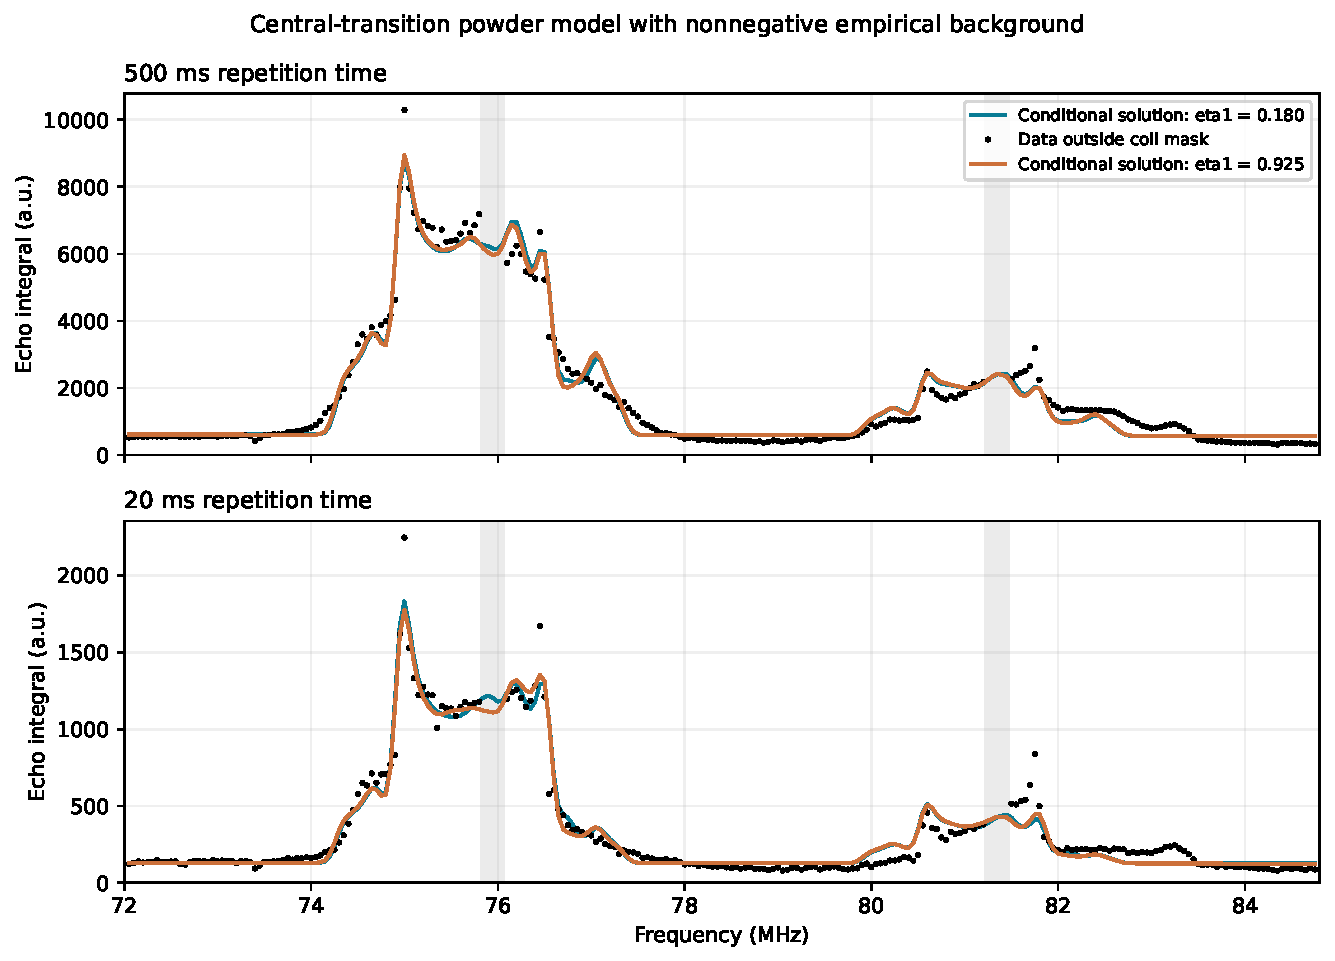
\includegraphics[width=0.88\textwidth]{figures/powder_model_comparison.pdf}
\caption{Joint description of the spectra at 500 and 20~ms repetition periods. Symbols are archived frequency-stepped echo integrals. Curves show the two central-transition solutions with nonnegative underlying terms in Table~\ref{tab:fit}. Gray bands mark the masked metallic-copper probe regions. The close agreement between the two model curves illustrates the ambiguity of the weakest spectral group's asymmetry.}
\label{fig:powder}
\end{figure*}

The first group is weakly constrained: markedly different $\eta_1$ values accompany comparable descriptions of both spectra. Within the tested isotropic-shift families, s2 remains near the axial limit, s3 gives $\eta\simeq0.18$--0.22, and s4 gives approximately 0.30--0.34. These ranges describe variation among fitted models. They are not statistical uncertainty intervals and do not include the effects of an unknown anisotropic shift tensor.

Repeating the joint all-transition comparison with the 2013 NQR set preserves both a smaller- and a larger-$\eta_1$ branch. Thus, the ambiguity is not removed by substituting the nearby published frequencies. A possible residual covellite contribution, whose $^{63}$Cu NQR frequency near 14.87~MHz is close to s2, and the actual pulsed-echo excitation profile remain additional physical considerations.

The effective Zeeman centers in Table~\ref{tab:fit} express the allowed differences in isotropic magnetic shifts. They are not calibrated Knight shifts. An absolute shift determination requires a consistent reference and allowance for the shift of metallic copper itself \citep{Locher1974,Harris2001}. Likewise, $\sigma$ is a phenomenological profile-convolution width and is not converted into an echo-decay time.

\subsection{Repetition-period dependence}

The change between the 20 and 500~ms spectra demonstrates that different parts of the observed envelope do not share the same recovery or excitation behavior. Ratios of summed archived integrals in broad windows 75.20--75.70 and 76.10--76.40~MHz are 5.73 and 4.71, respectively. These ratios are descriptive and are not converted into $T_1$ values without a recovery model.

Earlier zero-field NQR measurements at 4.2~K gave $^{63}T_1=0.200$ and 0.400~s for s2 and s4 \citep[p.~27]{Evlampiev2009}. They provide a useful relaxation scale, but the different field, transitions, and excitation conditions prevent a direct identification with the repetition-period dependence of the NMR spectra.

\section{Echo decay}

\subsection{Time scale and measured amplitude}

A separate archived dataset contains 35 echo-decay points recorded at 5~K, 51~MHz, and a nominal field of 45.7~kOe, approximately 4.57~T. Its variable \texttt{TwoTau} ranges from 40 to 1264.14. The old graph carries an inconsistent \texttt{mS} label. Here the numerical values are interpreted in microseconds, using the experimental context and the pulse and delay scales documented in the thesis \citep[pp.~18 and 29]{Evlampiev2009}. The echo time is explicitly defined as $t=2\tau$, so the recorded range extends to approximately 1.264~ms. This is a reconstructed unit convention for the archived dataset.

The original graph plots the imaginary part of the echo integral. Its complex phase changes from approximately $67^\circ$ to $50^\circ$ across the series; a single quadrature therefore also reflects a phase rotation. The principal amplitude used here is
\begin{equation}
E(t)=\sqrt{[\mathrm{IntRe}(t)]^2+
[\mathrm{IntIm}(t)]^2},
\label{eq:echo}
\end{equation}
which is invariant under a uniform rotation of the integrated quadratures. The separately stored \texttt{IntQ} column is not equal to Eq.~\eqref{eq:echo} and is analyzed only as an alternative amplitude definition.

\subsection{Effective envelope time}

The principal fit uses a generalized exponential with zero offset,
\begin{equation}
E(t)=A\exp\!\left[-\left(\frac{t}{\twe}\right)^\beta\right],
\qquad t=2\tau.
\label{eq:t2}
\end{equation}
For all 35 observations, $\twe=0.955$~ms and $\beta=1.26$. The parameter $\twe$ is the time at which the model envelope reaches $A/e$. A single exponential gives a similar time, 0.945~ms, but a larger root-mean-square residual: 25.93 rather than 7.89 arbitrary amplitude units. The exponent describes the envelope shape and does not by itself establish a microscopic relaxation mechanism.

\begin{figure*}[t]
\centering
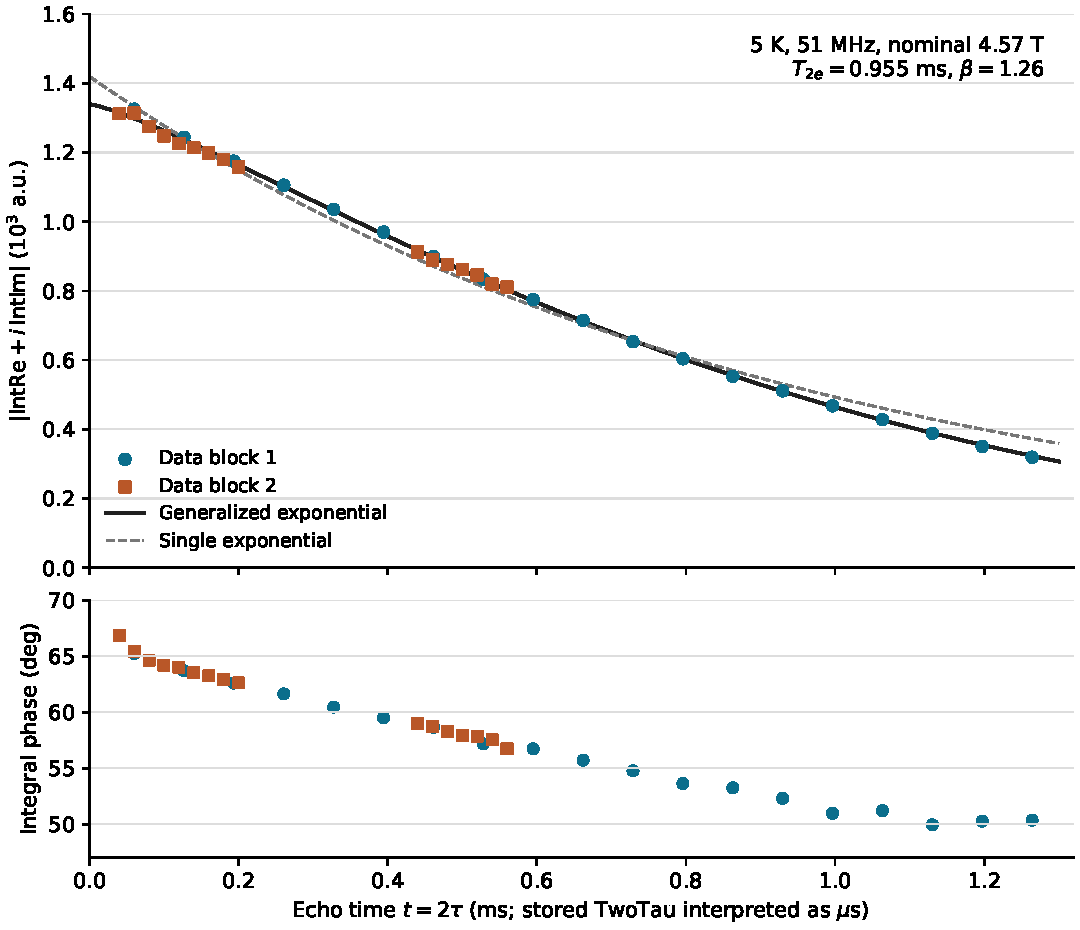
\includegraphics[width=0.86\textwidth]{figures/figure_t2_reanalysis.pdf}
\caption{Magnitude and phase of the complex echo integral in the separate 5~K, 51~MHz dataset. Different symbols indicate the two consecutive data blocks in the archived table. The generalized-exponential and single-exponential descriptions are compared. The numerical \texttt{TwoTau} values are interpreted in microseconds, with $t=2\tau$; the plotted time axis is in milliseconds.}
\label{fig:t2}
\end{figure*}

Fitting the data blocks separately and changing the early-time cutoff within the same generalized model gives times of approximately 0.94--1.00~ms. The second block ends at 560~$\mu$s, so its $1/e$ time is less directly constrained. Alternative amplitude definitions give 0.852~ms for the imaginary integral and 1.009~ms for the stored \texttt{IntQ}. These comparisons quantify sensitivity to processing, not statistical confidence limits. The principal result is therefore reported as an effective envelope time of approximately 0.95~ms.

The earlier NQR relaxation plot explicitly identifies $^{63}$Cu and labels its ordinate $T_2^{-1}$ in ms$^{-1}$ \citep[p.~29, Fig.~11]{Evlampiev2009}. Numerical tables have now been recovered directly from the embedded Origin object in the thesis. For the archived s3 group, rates at 6, 7, 8, 9, and 10~K are 7.070, 8.108, 7.709, 8.281, and 8.220~ms$^{-1}$, respectively, corresponding to $T_2\simeq0.121$--0.141~ms. At 6~K the stored rate-error column gives 0.297~ms$^{-1}$; its statistical definition is not independently documented. The separate covellite entry at 4.2~K is 9.094~ms$^{-1}$ and must not be assigned to anilite. The recovered s1, s2, and s4 tables begin at 77~K. These numerical records replace the earlier approximate reading of the plotted points and are preserved with their object-stream provenance. Their difference from the present NMR envelope time cannot be attributed to the external field alone without accounting for transition selection, spectral position, temperature, and pulse conditions.

\section{Crystallographic interpretation and assignment limits}

\subsection{What the spectra constrain}

The four high-frequency NQR doublets establish four resolved copper EFG environments in the component under reconsideration. The corresponding powder NMR envelope adds sensitivity to EFG asymmetry. It is therefore possible to constrain the local electronic environments while the crystallographic assignment remains unresolved.

In a nonoriented powder, $\eta$ is encoded in the complete distribution of transition frequencies, rather than in the value of one peak height. At fixed $\nu_{\nqr}$, changing $\eta$ changes both $\nuq$ through Eq.~\eqref{eq:nqr} and the angular variation of the transitions. Characteristic edges, shoulders, and intensity redistributions must then be reproduced simultaneously. In the present mixture, four such profiles overlap. The fitted parameters belong to the NQR-labeled spectral groups and cannot be assigned to Cu1--Cu5 merely by ordering their frequencies.

The reference room-temperature structure contains five Cu sites with multiplicities in the ratio $1:1:1:2:2$ \citep{Koto1970}. Expanding the published coordinates and symmetry operations gives the environments in Table~\ref{tab:structural}. Cu1 and Cu3 are tetrahedrally coordinated, whereas Cu2, Cu4, and Cu5 have three nearest sulfur neighbors. The fourth neighbor of Cu4 is substantially farther away, at approximately 2.94~\AA. The resulting count of eight tetrahedrally and twenty triangularly coordinated Cu atoms per cell agrees with the crystallochemical comparison of Evans \citep{Evans1981}.

Thus, the four high-frequency NQR groups cannot all be assigned to four distinct triangular sites of unchanged $Pnma$ anilite: that reference structure has only three such sites. If each group corresponds to a different site of this phase, at least one must involve a tetrahedral environment. A change of low-temperature symmetry or contributions from another phase would require a different counting argument.

Cu1--Cu3 occupy Wyckoff position $4c$ with mirror site symmetry $.m.$; Cu4 and Cu5 occupy general positions $8d$ with site symmetry $1$. None of these symmetries requires $\eta=0$. At a mirror site, invariance under reflection perpendicular to $b$ gives $V_{ab}=V_{bc}=0$. The $b$ direction is therefore an EFG principal direction, but symmetry neither selects it as the direction of the largest principal value nor requires the other two eigenvalues to be equal.

These multiplicities are population constraints, not automatically measured spin-echo intensity ratios. Relaxation, excitation bandwidth, pulse efficiency, overlap, and instrumental frequency response affect the observable amplitudes.

X-ray diffraction supplies atomic coordinates, occupancies, displacement parameters, and symmetry. Numerical EFG asymmetries additionally require the local charge distribution. They cannot generally be identified with a bond-length distortion or an atomic displacement parameter. The structural reference used here is the near-room-temperature coordinate set archived as AMCSD~0009376, rather than a verified diffraction refinement of the present material at 5~K.

\subsection{Exploratory electrostatic model}

To assess what the reference geometry might suggest, a separate point-charge calculation was performed without using the NMR fit parameters. Define the geometrical tensor
\begin{equation}
G_{\alpha\beta}
=\sum_{j,\bm R}'q_j
\frac{3r_{j,\alpha}r_{j,\beta}
-r_j^2\delta_{\alpha\beta}}{r_j^5},
\label{eq:pointcharge}
\end{equation}
where the sum includes periodic images, $q_j$ is expressed in units of the elementary charge, and the observation-site self term is omitted. A Coulomb prefactor would convert $G$ to an electrostatic field gradient, but the full nuclear EFG also contains electronic contributions not represented in this model.

The baseline model assigns $q_{\Cu}=8/7$ and $q_{\mathrm S}=-2$, ensuring neutrality of the 28-Cu, 16-S unit cell. These are trial charges, not an experimental oxidation-state assignment. Periodic sums were evaluated by the Ewald method and checked by varying the splitting parameter and comparing with direct finite-radius sums. Additional neutral scenarios start from $q_{\Cu}=1$ and assign the remaining four positive charge units to one Cu orbit at a time: the charge increment on that orbit is $4/m_s$, where $m_s$ is its unit-cell multiplicity. All coordinates are held fixed.

\begin{table*}[t]
\centering
\small
\setlength{\tabcolsep}{4pt}
\caption{Crystallographic reference and exploratory point-charge results. Site labels and coordinates follow the room-temperature Koto--Morimoto structure \citep{Koto1970}; coordination and the numerical columns were calculated here. $\eta_{\rm pc}$ describes $G$; it is not an experimental determination or an electronic-structure prediction of the nuclear-EFG asymmetry. The relative magnitude is normalized to Cu2 in the uniform-Cu-charge model. The final column spans six chosen neutral charge scenarios and is not an experimental uncertainty interval.}
\label{tab:structural}
\begin{tabular}{llrlrrr}
\toprule
Site & Wyckoff / symmetry & $m_s$ & Nearest-S coordination
& $\eta_{\rm pc}$ & $|G_{ZZ}|/|G_{ZZ}^{\Cu2}|$
& Scenario span of $\eta_{\rm pc}$ \\
\midrule
Cu1 & $4c$ / $.m.$ & 4 & Distorted tetrahedral & 0.557 & 0.688 & 0.095--0.774 \\
Cu2 & $4c$ / $.m.$ & 4 & Nearly regular triangular & 0.059 & 1.000 & 0.018--0.165 \\
Cu3 & $4c$ / $.m.$ & 4 & Tetrahedral & 0.255 & 0.088 & 0.069--0.842 \\
Cu4 & $8d$ / $1$ & 8 & Triangular & 0.163 & 0.847 & 0.035--0.537 \\
Cu5 & $8d$ / $1$ & 8 & Distorted triangular & 0.585 & 0.951 & 0.566--0.642 \\
\bottomrule
\end{tabular}
\end{table*}

The baseline values in Table~\ref{tab:structural} should be read as hypotheses generated by a specified electrostatic model. They omit the on-site electronic charge distribution, covalency, screening, and antishielding. Numerical convergence of the lattice sum does not remove this physical limitation, and its magnitude is not converted into predicted NQR frequencies.

Two tendencies are useful for designing an assignment test. First, Cu2 has a nearly regular triangular environment and a small model asymmetry. It is a plausible candidate for a nearly axial contribution, but matching this single number is insufficient: Cu2 also has one of the largest model $|G_{ZZ}|$, whereas the near-axial fitted group s2 is not the highest-frequency NQR group. Frequencies and asymmetries must be matched together.

Second, Cu3 has a much smaller model tensor magnitude than the other four sites. It remains the smallest in all six charge scenarios, motivating a possible low-EFG contribution from this tetrahedral site. This is consistent with investigating an overlapping or low-frequency fifth response, but does not identify an observed resonance or establish a frequency for it. A nearly regular tetrahedron should not be equated with $\eta\simeq0$: exact tetrahedral symmetry makes the entire EFG vanish, whereas a small residual tensor can have a sizeable and model-sensitive asymmetry.

The sensitivity is substantial even within this elementary approach. For Cu1, the nearest sulfur shell alone gives $\eta_{\rm pc}\simeq0.021$, while the complete periodic baseline model gives 0.557. Geometry of the first coordination shell is therefore insufficient even before electronic EFG contributions are considered. A quantitative crystallographic assignment requires an electronic-structure EFG calculation and comparison with the complete experimental spectrum.

An additional conditional scale test defines $P_s=|G_{ZZ,s}|\sqrt{1+\eta_{{\rm pc},s}^2/3}$ and fits one common positive multiplier to the four high-frequency NQR values. All 24 assignments to Cu1, Cu2, Cu4, and Cu5 are retained for each charge scenario; Cu3 is withheld from the calibration. The best frequency-only match in the uniform-charge model places the scaled Cu3 response at 1.503~MHz, close to the lower end of the archived low-frequency interval. The corresponding best matches across the six scenarios span 1.40--3.52~MHz.

This empirical scaling assumes a common conversion for all five sites and is not an independent prediction of an absolute nuclear EFG. Even the baseline match leaves a high-frequency root-mean-square residual of 0.584~MHz, with a maximum relative residual of 6.07\%, and does not reproduce the NMR-derived asymmetries. The comparison therefore motivates a targeted low-frequency assignment test without selecting an established charge distribution or a Cu-site mapping. All 144 assignments and their frequency and asymmetry discrepancies are retained in the supporting calculations.


% Manuscript-ready fragment. Bibliography keys: Evlampiev2009, Gainov2010.
% Archival evidence and subsequent author recollection are explicitly separated.
\subsection{Low-frequency NQR evidence}

The thesis explicitly reports copper NQR signals at 4.2~K in the
1.5--2.2~MHz interval \citep[p.~22]{Evlampiev2009}.
Its Fig.~8, captioned for a sample of nominal composition
Cu$_{1.1}$S, shows both a frequency-stepped spin-echo spectrum and an
FT-based reconstruction \citep[p.~23]{Evlampiev2009}.
The nominal composition describes a mixed synthetic sample, rather than
the stoichiometry of an individual anilite phase.
The thesis states that broadening and overlap prevented separation of
the component then called geerite from covellite and prevented a count
of the corresponding inequivalent Cu sites.
Its discussion already tentatively associated the low-frequency response
with tetrahedrally coordinated copper \citep[p.~33]{Evlampiev2009}.
The spectrum was therefore not assigned in its entirety to an unknown
extraneous impurity.

A related review retained the tentative entry ``Site~?'' and
``Below 2~MHz?'' for the material then called geerite
\citep[Table~I, p.~332]{Gainov2010}.
The same source gives the covellite low-frequency pair at 1.87 and
1.73~MHz for $^{63}$Cu and $^{65}$Cu, respectively, at 4.2~K.
Consequently, the archived low-frequency intensity cannot be attributed
entirely to anilite.

The experimenter additionally reports that the low-frequency
instrumentation and resonant circuits had not been sufficiently optimized in
this range for a detailed investigation (author communication,
27 November 2026). This recollection supplements the archive:
the thesis lists a nominal 1--32~MHz low-frequency spectrometer, but its
explicit reason for not resolving the low-frequency components is their
width and overlap.
The earlier publication independently documents an effective lower
frequency limit of about 1.5~MHz and reports that the covellite
low-frequency response could be followed only up to 30~K
\citep{Gainov2009}. This published operating limit supports the existence
of instrumental constraints, while the recollection about circuit
optimization remains a separate source of information.

Under the revised phase identification, the small model EFG at Cu3
provides a site-specific hypothesis for a possible anilite contribution
within this previously observed interval. It does not establish the
frequency of Cu3, resolve its isotope pair, or quantify its contribution
to the mixed spectrum. The observation supports a targeted assignment
test while retaining covellite as a known overlapping response.


\subsection{What NQR and temperature variation add}

For a spin-$3/2$ isotope there is only one zero-field NQR frequency for each distinct EFG environment. Equation~\eqref{eq:nqr} therefore leaves a continuous relation between $|V_{ZZ}|$ and $\eta$. The second copper isotope largely supplies the expected quadrupole-moment scaling and strengthens the identification of a copper pair; it does not provide an independent equation that uniquely separates these two EFG quantities.

Likewise, a temperature-dependent NQR frequency tracks a combination of EFG magnitude and asymmetry. With temperature-independent nuclear constants,
\begin{equation}
\frac{d\ln\nu_{\nqr}}{dT}
=\frac{d\ln|V_{ZZ}|}{dT}
+\frac{\eta}{3+\eta^2}\frac{d\eta}{dT}.
\label{eq:temperature}
\end{equation}
Frequency shifts alone therefore do not determine $\eta(T)$.

A useful magnitude constraint nevertheless follows without a fitted asymmetry. Since $0\leq\eta\leq1$,
\begin{equation}
\frac{\sqrt{3}}{2}\nu_{\nqr}\leq|\nu_Q|\leq\nu_{\nqr}.
\label{eq:nqrbound}
\end{equation}
The s1 and s4 frequencies give disjoint intervals, 10.366--11.970 and 14.688--16.960~MHz, respectively. Hence $|V_{ZZ,\mathrm{s4}}|/|V_{ZZ,\mathrm{s1}}|\geq1.227$. The observed frequency spread cannot be explained by different asymmetries at a single common EFG magnitude.

The earlier thesis reports that the four high-frequency NQR branches are nearly temperature independent below approximately 50--65~K and decrease more rapidly above this range \citep[pp.~23--24]{Evlampiev2009}. The s1--s3 branches have similar trends, whereas s4 decreases faster and crosses s3 near 200~K. The thesis described the feature near 55~K as a transition of the component then called geerite. With the revised phase assignment, these observations motivate an EFG anomaly or crossover in the anilite-related component. A symmetry-changing transition remains a candidate interpretation rather than a diffraction-established result: the available frequency curves do not separate $V_{ZZ}(T)$ from $\eta(T)$.

The recovered Origin temperature project also contains columns labeled for $^{65}$Cu that are numerically generated from the corresponding $^{63}$Cu columns by division by 1.081. Those constructed columns are retained with their provenance and are not counted as independent isotope-resolved temperature measurements.

The low-temperature covellite structure discussed in the earlier work, including its symmetry change, belongs to CuS and must not be transferred to anilite. A useful anilite assignment would compare EFG tensors calculated for its own crystallographic sites with the complete NQR frequency set, powder NMR line shapes, and their temperature evolution. The present single-temperature NMR analysis does not establish a Cu-site exchange process or site-resolved $\eta(T)$.

\subsection{Constraints from the spectral wings}

No additional resolved signal was observed beyond the measured wings. A proposed assignment must respect this observation and should not predict a sufficiently intense isolated resonance in such a region. However, an additional site need not generate an outer-wing feature.

For example, direct diagonalization with $\nuz=76$~MHz, $\nu_{\nqr}=1.5$~MHz, and $\eta=0$ puts the central transition between approximately $-9.9$ and $+5.6$~kHz relative to $\nuz$, while the satellite transitions lie within 74.5--77.5~MHz. At $\eta=1$, the central-transition interval is approximately $-14.8$ to $+7.4$~kHz. Such a component could overlap the existing broad response and lie close to the probe-copper region.

This numerical example demonstrates a limit of the inference from absent outer wings; it does not identify a fifth anilite resonance. Neither does the unresolved low-frequency NQR response of the earlier mixed sample establish that assignment. The difference between five crystallographic sites and four resolved high-frequency doublets must therefore be addressed through overlap, visibility, and independent EFG constraints, rather than by equating the two counts.

\section{Conclusions}

The revised phase identification connects earlier NQR data, described first as geerite and later as digenite, with powder NMR measurements on anilite. The absence of particle alignment and the common NQR/NMR material are incorporated directly into the analysis. Metallic-copper probe signals are handled as an ordinary instrumental contribution.

Joint powder-spectrum fits constrained by four NQR pairs provide conditional quadrupolar parameters. Within the tested isotropic-shift models, s2 is close to the axial limit, s3 gives $\eta$ near 0.18--0.22, and s4 near 0.30--0.34. Comparable smaller- and larger-$\eta_1$ solutions show that the weakest group's asymmetry is not uniquely established. These spectral-group parameters do not yet determine a Cu1--Cu5 assignment. The reference structure has only three triangular Cu sites, so an assignment of all four groups to distinct triangular environments is incompatible with unchanged $Pnma$ anilite. The point-charge comparison motivates a small-EFG Cu3 hypothesis but is not an electronic EFG prediction.

A separate echo-decay series yields an effective complex-envelope time of approximately 0.95~ms after reconstructing the microsecond time scale. Recovered s3 NQR tables give $T_2\simeq0.12$--0.14~ms at 6--10~K. Their joint interpretation must retain the different transition and excitation conditions. The revised assignment, explicit powder modeling, and preserved ambiguity together provide a basis for a crystallographically constrained interpretation of the copper environments.

\section*{Data and calculation availability}

The archived input files, extracted integral tables, fitting scripts, numerical powder profiles, alternative-model results, and echo-decay calculations are preserved in the \href{https://github.com/Eljah/nmr_CuS/tree/master}{\texttt{Eljah/nmr\_CuS} repository, branch \texttt{master}}. Embedded Origin objects recovered from the supplied thesis and document files are retained byte for byte, together with their numerical exports and provenance. The repository distinguishes the final model-comparison table from preliminary fits and retains the earlier manuscript snapshot.

A companion theoretical supplement, \texttt{theory/efg\_derivation.tex}, derives the Coulomb Hessian, periodic Ewald terms and self correction, spin-$3/2$ quadrupolar levels, powder averaging, and the small-EFG central-transition limit. Symbolic checks and numerical intermediate records include expanded atomic sites, all retained real- and reciprocal-space tensor contributions, subtotal tensors, eigensystems, convergence tests, and conditional frequency-scaling comparisons. The reported numerical precision is chosen for physical interpretation; additional digits in machine-readable files describe calculations rather than experimental accuracy.

\bibliographystyle{unsrtnat}
\bibliography{references}

\end{document}
